\section{Apartado D}


\subsection{Diagrama de Diseño}

\begin{figure}[H]
    \centering
     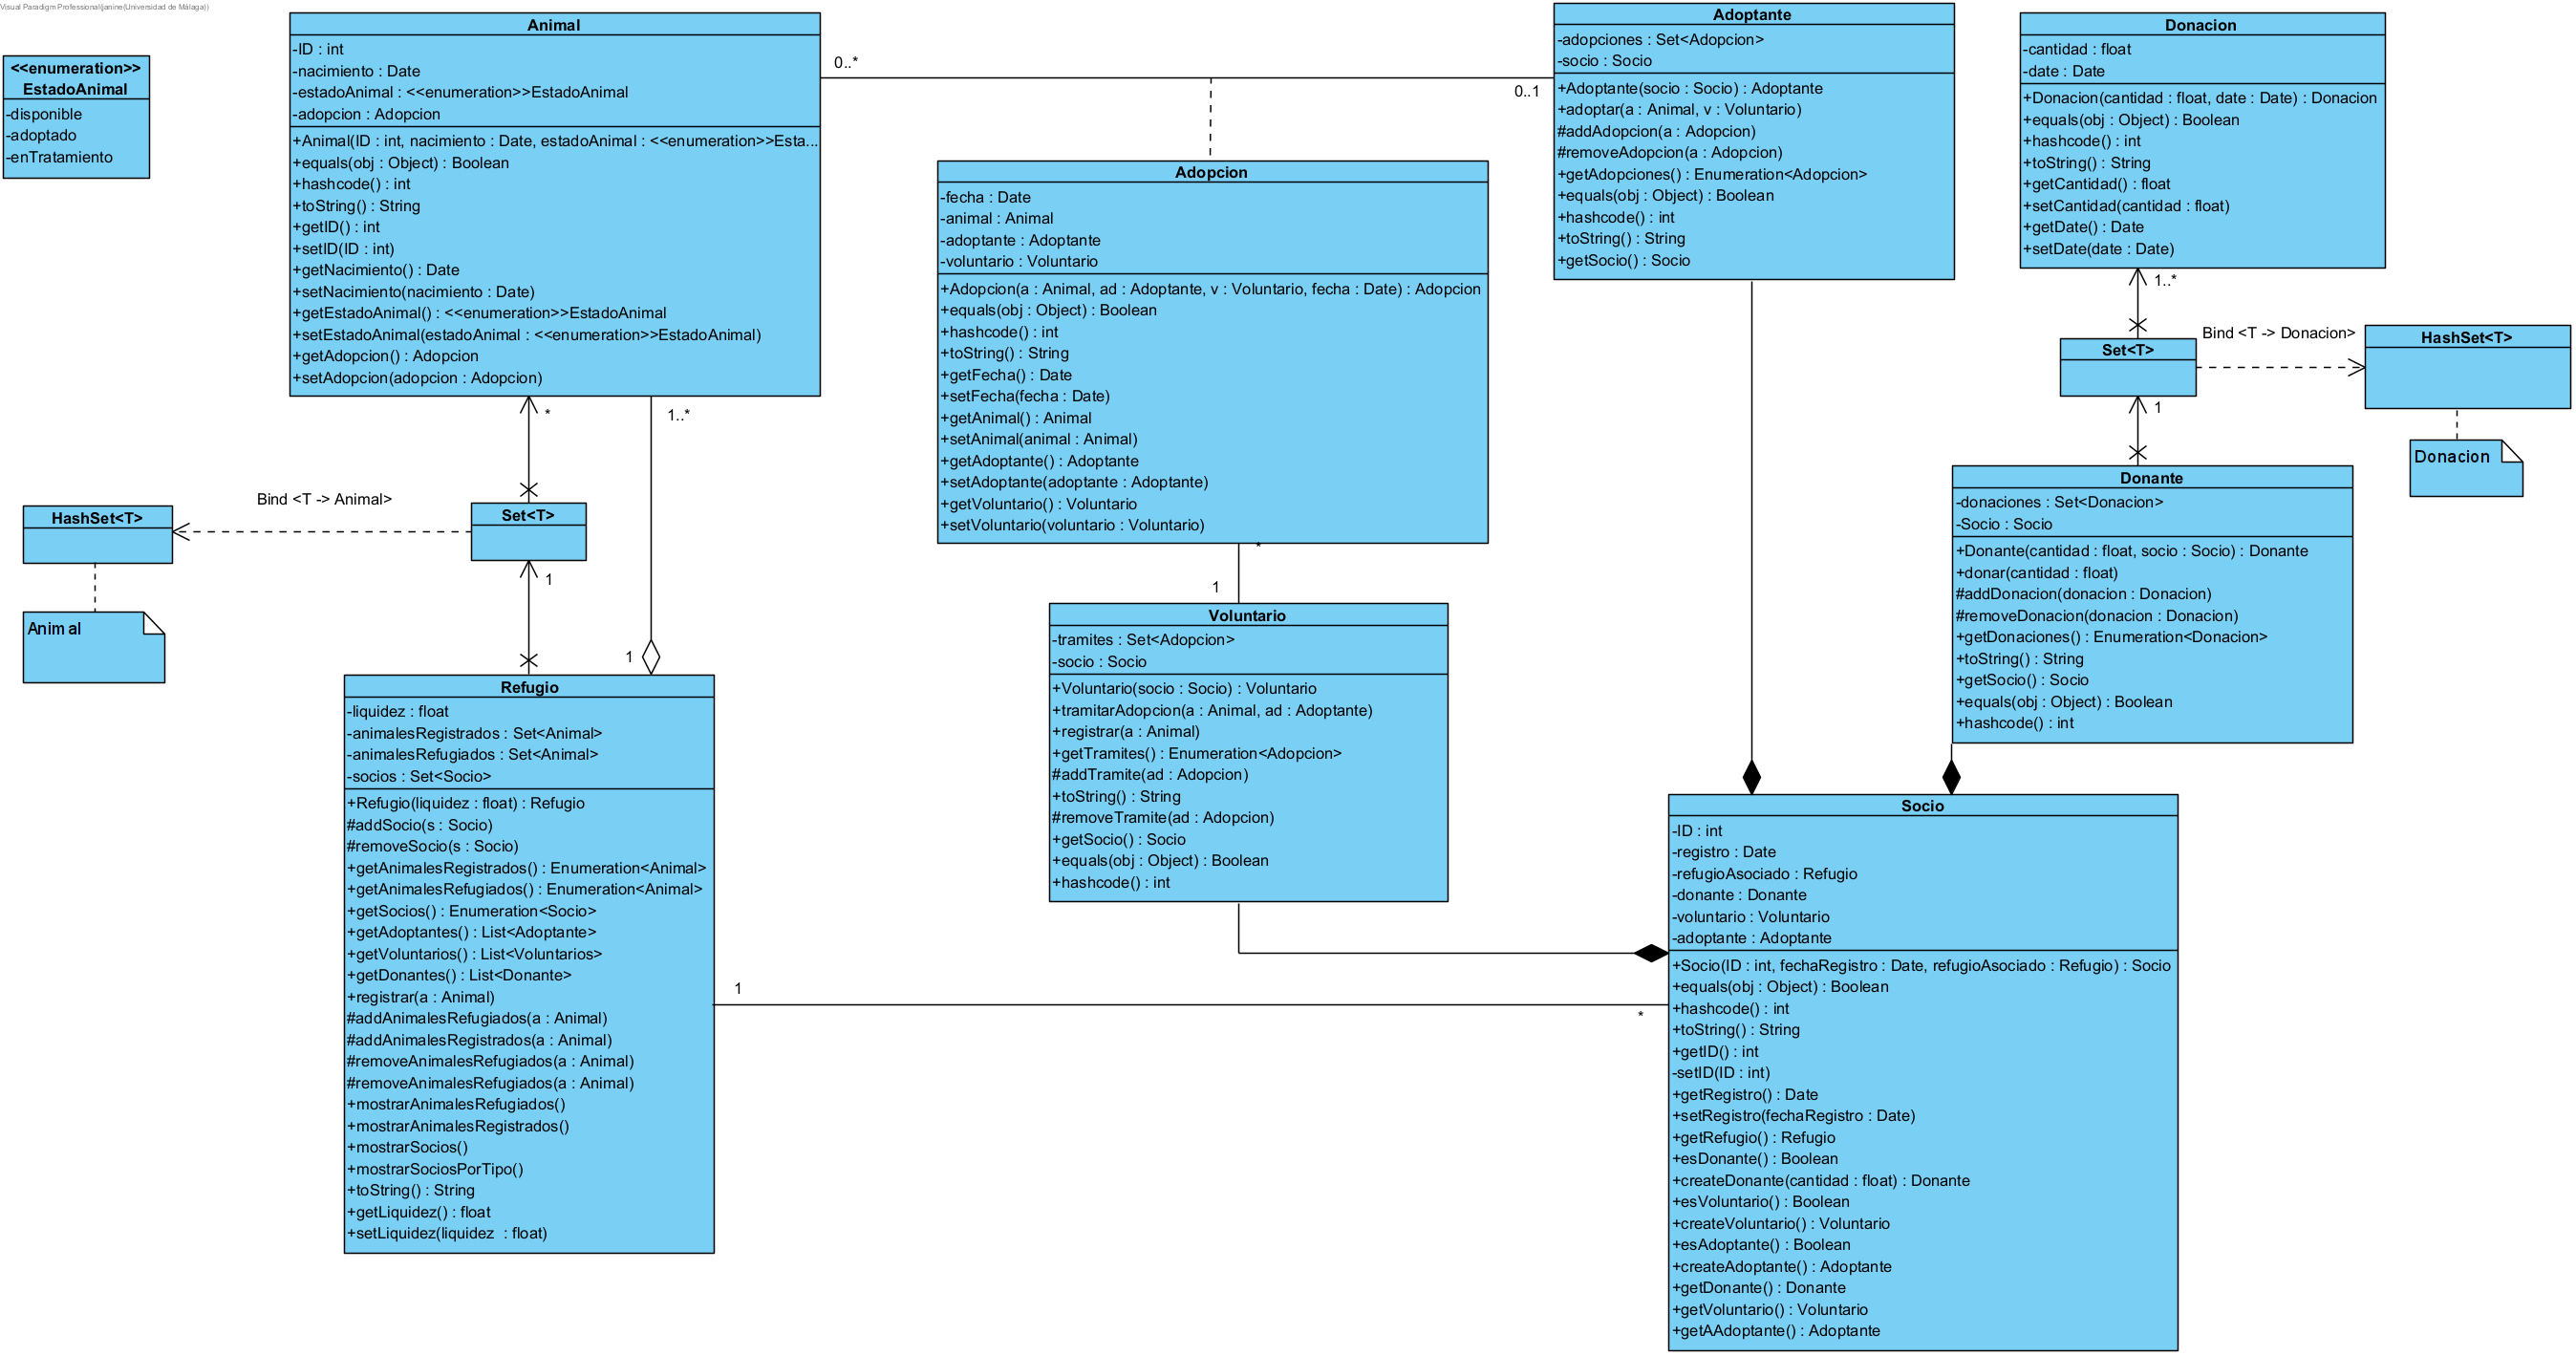
\includegraphics[width=1\linewidth]{assets/Class Diagram1.png}
     \caption{Diagrama de Diseño del apartado D}
\end{figure}

\subsection{Solución propuesta}
Hemos decido implementarlo por composición por las siguientes razones:
\begin{itemize}
    \item \textbf{Menor Acoplamiento:} Reduce la dependencia directa entre clases principales porque ahora se distribuimos responsabilidades a clases especificas.
    \item \textbf{Evita Problemas de Herencia:} A diferencia de la herencia implementada originalmente, como se discutió, la composición no impone una estructura rígida.
\end{itemize}

Ahora, las clases pueden combinar comportamientos dinámicamente como se ve a continuación:
\begin{lstlisting}[style = javaNormal, language=Java] 
package sistema;

import java.util.Collections;
import java.util.Date;

public class Socio {
    private int ID;
    private Date registro;
    private final Refugio refugioAsociado;

    private Donante donante;
    private Voluntario voluntario;
    private Adoptante adoptante;

    public Socio(int ID, Date fechaRegistro, Refugio refugioAsociado) {
        assert ID > 0 : "El ID del socio debe ser valido.";
        assert fechaRegistro != null : "La fecha de registro no puede ser nula.";
        assert refugioAsociado != null : "El refugio asociado no puede ser nulo.";

        this.ID = ID;
        this.registro = fechaRegistro;
        this.refugioAsociado = refugioAsociado;
        refugioAsociado.addSocio(this);

        assert refugioAsociado.getSocios().hasMoreElements() && Collections.list(refugioAsociado.getSocios()).contains(this);
    }
    public int getID(){
        return ID;
    }
    private void setID(int ID){
        assert ID > 0;
        assert Collections.list(this.getRefugio().getSocios()).stream().noneMatch(s -> s.getID() == ID)
            : "El ID ya existe en el refugio";
        this.ID = ID;
    }
    public Date getRegistro() {
        return this.registro;
    }
    public void setRegistro(Date fechaRegistro) {
        assert  fechaRegistro != null;
        this.registro = fechaRegistro;
    }
    public Refugio getRefugio() {
        return this.refugioAsociado;
    }

    public boolean esDonante() {
        return this.donante != null;
    }
    public Donante createDonante(float cantidad) {
        this.donante = new Donante(cantidad, this);
        return this.donante;
    }
    public boolean esVoluntario() {
        return this.voluntario != null;
    }
    public Voluntario createVoluntario() {
        this.voluntario = new Voluntario(this);
        return this.voluntario;
    }
    public boolean esAdoptante() {
        return adoptante != null;
    }
    public Adoptante createAdoptante() {
        this.adoptante = new Adoptante(this);
        return this.adoptante;
    }

    public Donante getDonante() {
        return donante;
    }

    public Voluntario getVoluntario() {
        return voluntario;
    }

    public Adoptante getAdoptante() {
        return adoptante;
    }

    @Override
    public boolean equals(Object obj) {
        if( this == obj ) return true;
        if(obj instanceof Socio ){
            Socio socio = (Socio) obj;
            return this.ID == socio.ID;
        }
        return false;
    }

    @Override
    public int hashCode() {
        return Integer.hashCode(ID);
    }
    @Override
    public String toString() {
        return "Socio{" +
                "ID=" + ID +
                ", registro=" + registro +
                ", donante=" + donante +
                ", voluntario=" + voluntario +
                ", adoptante=" + adoptante +
                '}';
    }
}

\end{lstlisting}

\subsection{Cambios respecto a la implementación original}
En nuestra implementación, las clases que anteriormente heredaban de \texttt{Socio} ahora se relacionan con esta mediante 
una \textbf{composición bidireccional}. Este enfoque reemplaza la jerarquía de herencia propuesta originalmente por una 
estructura más flexible, donde la clase \texttt{Socio} incluye atributos que representan las relaciones con \texttt{Adoptante}, 
\texttt{Voluntario} y \texttt{Adoptante}. De manera similar, cada clase de rol contiene un atributo que apunta a una instancia 
de la clase \texttt{Socio}, estableciendo un vínculo mutuo y permitiendo una interacción más modular y adaptable.

Para gestionar los roles, la clase \texttt{Socio} incluye métodos booleanos que permiten verificar si una instancia es 
\texttt{Adoptante}, \texttt{voluntario} o \texttt{Donante}, basándose en si el atributo correspondiente está instanciando 
o es null. Si un socio no tiene asignado un rol, el atributo asociado permanecerá null, indicando que no desempeña dicha 
función. Además, para facilitar la adopción de nuevos roles, se han añadido métodos que crean instancias de las clases 
correspondientes y asignan estos objetos a los atributos de la clase Socio, asegurando una inicialización controlada y 
coherente de los roles.

\subsubsection{Constructores de cada rol}
Originalmente, cada constructor necesitaba llamar a la clase padre para obtener sus atributos específicos, extendiendo con su comportamiento especifico.
Ahora como no tenemos esa distinción, \texttt{Socio} es el objeto que contiene toda la información relevante, entonces en los constructores es el único parámetro.
Además, como solo puede existir un sólo tipo de objeto (\texttt{Socio}), en cada clase con métodos específicos al rol de éste, se define como un atributo \emph{private final}.

\begin{lstlisting}[style = javaNormal, language=Java, caption={extracto de la clase Adoptante}] 
    [...]
    private final Socio socio;
    //Constructor para un adoptante
    public Adoptante(Socio socio) {
        adopciones = new HashSet<>();
        this.socio = socio;
    }
    [...]
\end{lstlisting}

Todos los cambios presentes se encuentran también en las clases \texttt{Donante}, \texttt{Voluntario}.

\subsubsection{Métodos hashCode y equals}
En la primera implementación las comprobaciones de igualdad se realizan viendo si el objeto era del mismo tipo, y el \texttt{ID} del \texttt{Socio} que heredan es el mismo.
Ahora como hemos eliminado la herencia, las comprobaciones se hacen directamente con la instancia del tipo correspondiente y su socio asociado; si tienen el mismo ID se consideran el mismo objeto.

\begin{lstlisting}[style = javaNormal, language=Java, caption={extracto de la clase Adoptante}]
    [...] 
    //Metodo que comprueba si dos adoptantes son iguales
@Override
public boolean equals(Object obj) {
    if (this == obj) return true;
    if(obj instanceof Adoptante ){
        Adoptante adoptante = (Adoptante) obj;
        return getSocio().getID() == this.getSocio().getID(); 
    }
    return false;
}
@Override
public int hashCode() {
    return Integer.hashCode(getSocio().getID());
}
[...]
\end{lstlisting}

Todos los cambios presentes se encuentran también en las clases \texttt{Donante}, \texttt{Voluntario}.

\subsubsection{Manejo de las estructuras de datos}
En la clase Refugio, se ha simplificado la estructura al eliminar los conjuntos específicos para Adoptante, 
Voluntario y Donante, sustituyéndolos por un único Set<Socio> que centraliza la gestión de todos los socios. 
Para agregar o eliminar socios, se han implementado los métodos addSocio y removeSocio, que mantienen la integridad del 
conjunto. Adicionalmente, se han incorporado métodos públicos que devuelven listas filtradas por tipo de rol (adoptante, 
voluntario o donante). Estos métodos verifican dinámicamente los roles de los socios dentro del conjunto, garantizando 
que solo se incluyan aquellos que cumplan con los criterios específicos.

\begin{lstlisting}[style = javaNormal, language=Java, caption={extracto de la clase Refugio}] 
    [...]
    public List<Adoptante> getAdoptantes() {
        List<Adoptante> adoptantes = new ArrayList<>();
        for (Socio s : socios) {
            if (s.esAdoptante()) {
                adoptantes.add(s.getAdoptante());
            }
        }
        return adoptantes;
    }

    public List<Voluntario> getVoluntarios() {
        List<Voluntario> voluntarios = new ArrayList<>();
        for (Socio s : socios) {
            if (s.esVoluntario()) {
                voluntarios.add(s.getVoluntario());
            }
        }
        return voluntarios;
    }

    public List<Donante> getDonantes() {
        List<Donante> donantes = new ArrayList<>();
        for (Socio s : socios) {
            if (s.esDonante()) {
                donantes.add(s.getDonante());
            }
        }
        return donantes;
    }
    [...]
\end{lstlisting}

Esta estructura centralizada y modular mejora la eficiencia, reduce la redundancia en la gestión de datos y facilita la 
extensión del sistema para incluir nuevos roles o funcionalidades en el futuro.

\subsubsection{Acceso a los datos}
Cada una de las clases \enquote{rol} hacen acceso a la clase \texttt{Socio} mediante una instancia que alberga el siguiente método:

\begin{lstlisting}[style = javaNormal, language=Java] 
public Socio getSocio() {
        return socio;
    }
\end{lstlisting}


\subsection{Testing}
Con la siguiente clase hemos comprobado el funcionamiento del sistema:
\begin{lstlisting}[style = javaNormal, language=Java] 
    import sistema.*;

    import java.util.Date;
    
    public class Test {
        public static void main(String[] args) {
            System.out.println("Pruebas del sistema de refugio de animales\n");
    
            // Caso 1: Pruebas exitosas (configuracion y operaciones validas)
            try {
                System.out.println("Caso 1: Pruebas exitosas\n");
    
                // Crear un refugio con liquidez inicial
                Refugio refugio = new Refugio(500.00f);
                //Se ha asumido que solo se puede crear un refugio
    
                // Crear socios
                Socio socio = new Socio(1, new Date(), refugio);
                socio.createVoluntario();
    
                socio.createDonante(100.00f);
                socio.createAdoptante();
    
                Voluntario voluntario = socio.getVoluntario();
                Donante donante = socio.getDonante();
                Adoptante adoptante = socio.getAdoptante();
    
    
                
                // Registrar animales en el refugio
                //Se entiende que el estado de ENTRATAMIENTO es el estado en el que se encuentra un animal que no esta ni disponible ni adoptado
                Animal animal1 = new Animal(101, new Date(), EstadoAnimal.ENTRATAMIENTO);
                Animal animal2 = new Animal(102, new Date(), EstadoAnimal.ENTRATAMIENTO);
                voluntario.registrar(animal1);
                voluntario.registrar(animal2); 
                //Creo un socio asociado a otro refugio e intento meter el mismo animal
    
                // Donante realiza una donacion adicional
                donante.donar(50.00f);
                //Hasta aqui funciona el registro de socios, el meto do donar y el meto do registrar funcionan perfactemente.
                // Adoptante adopta un animal
                adoptante.adoptar(animal1, voluntario);
                //adoptante.adoptar(animal1, voluntario); Falla porque el animal ya ha sido adoptado
    
                // Mostrar estado final del refugio
                System.out.println(refugio.toString());
            } catch (Exception e) {
                System.out.println("Error en el Caso 1: " + e.getMessage());
            }
    
            // Caso 2: Pruebas de errores (fallos en los asserts)
            try {
                System.out.println("\nCaso 2: Adoptar dos veces el mismo animal\n");
    
                // Intentar registrar un animal nulo
                //Se ha asumido que solo se puede crear un refugio
    
                // Crear socios
    
                // Crear un refugio con liquidez inicial
                Refugio refugio = new Refugio(500.00f);
                //Se ha asumido que solo se puede crear un refugio
    
                //Crear socios
                Socio socio = new Socio(1, new Date(), refugio);
                socio.createVoluntario();
                socio.createDonante(100.00f);
                socio.createAdoptante();
    
                Animal animal1 = new Animal(101, new Date(), EstadoAnimal.ENTRATAMIENTO);
                Voluntario voluntario = socio.getVoluntario();
                Adoptante adoptante = socio.getAdoptante();
    
                voluntario.registrar(animal1);
    
                adoptante.adoptar(animal1, voluntario);
                adoptante.adoptar(animal1, voluntario);
    
                System.out.println(refugio.toString());
    
            } catch (AssertionError e) {
                System.out.println("Error detectado: " + e.getMessage());
            }
            // Caso 3: Intentar meter dos veces el mismo socio en el mismo refugio
            try {
                System.out.println("\nCaso 3: Intentar meter dos veces el mismo socio en el mismo refugio\n");
    
                // Crear un refugio con liquidez inicial
                Refugio refugio = new Refugio(500.00f);
    
                //Se ha asumido que solo se puede crear un refugio
                //Crear socios
                Socio socio = new Socio(1, new Date(), refugio);
                Socio socio2 = new Socio(1, new Date(), refugio);
    
                System.out.println(refugio.toString());
            } catch (AssertionError e) {
                System.out.println("Error detectado: " + e.getMessage());
            }
    
            // Caso 4:  Intentar que un socio sea dos voluntarios
            try {
                System.out.println("\nCaso 4: Intentar que un socio sea dos donantes, voluntarios y adoptantes\n");
    
                // Crear un refugio con liquidez inicial
                Refugio refugio = new Refugio(500.00f);
    
                //Se ha asumido que solo se puede crear un refugio
                //Crear socios
                Socio socio = new Socio(1, new Date(), refugio);
    
                socio.createVoluntario();
                socio.createDonante(100.00f);
                socio.createAdoptante();
    
                socio.createVoluntario();
                //socio.createDonante(1.00f);
                //socio.createAdoptante();
    
                System.out.println(refugio.toString());
            } catch (AssertionError e) {
                System.out.println("Error detectado: " + e.getMessage());
            }
    
            // Caso 5:  Intentar que un socio sea dos donantes
            try {
                System.out.println("\nCaso 5:  Intentar que un socio sea dos donantes\n");
    
                // Crear un refugio con liquidez inicial
                Refugio refugio = new Refugio(500.00f);
    
                //Se ha asumido que solo se puede crear un refugio
                //Crear socios
                Socio socio = new Socio(1, new Date(), refugio);
    
                socio.createVoluntario();
                socio.createDonante(100.00f);
                socio.createAdoptante();
    
                //socio.createVoluntario();
                socio.createDonante(1.00f);
                //socio.createAdoptante();
    
                System.out.println(refugio.toString());
            } catch (AssertionError e) {
                System.out.println("Error detectado: " + e.getMessage());
            }
            // Caso 6:  Intentar que un socio sea dos adoptantes
            try {
                System.out.println("\nCaso 6:  Intentar que un socio sea dos adoptantes\n");
    
                // Crear un refugio con liquidez inicial
                Refugio refugio = new Refugio(500.00f);
    
                //Se ha asumido que solo se puede crear un refugio
                //Crear socios
                Socio socio = new Socio(1, new Date(), refugio);
    
                socio.createVoluntario();
                socio.createDonante(100.00f);
                socio.createAdoptante();
    
                //socio.createVoluntario();
                //socio.createDonante(1.00f);
                socio.createAdoptante();
    
                System.out.println(refugio.toString());
            } catch (AssertionError e) {
                System.out.println("Error detectado: " + e.getMessage());
            }
    
            // Caso 7: Meter un animal dos veces en el mismo refugio, el mismo animal y luego dos distintos, desde refugio y desde voluntario
            try {
                System.out.println("\nCaso 7: Meter un animal dos veces en el mismo refugio, el mismo animal y luego dos distintos, desde refugio y desde voluntario\n");
    
                // Crear un refugio con liquidez inicial
                Refugio refugio = new Refugio(500.00f);
    
                //Se ha asumido que solo se puede crear un refugio
                //Crear socios
                Socio socio = new Socio(1, new Date(), refugio);
    
                Animal animal = new Animal(101, new Date(), EstadoAnimal.ENTRATAMIENTO);
                Animal animal2 = new Animal(102, new Date(), EstadoAnimal.ENTRATAMIENTO);
    
                Voluntario voluntario = socio.createVoluntario();
                voluntario.registrar(animal);
                voluntario.registrar(animal);
    
                refugio.registrar(animal2);
                refugio.registrar(animal2);
    
                System.out.println(refugio.toString());
            } catch (AssertionError e) {
                System.out.println("Error detectado: " + e.getMessage());
            }
        }
    }
    
\end{lstlisting}

\subsubsection{Output}

\begin{lstlisting}[style = javaNormal, language=Java]
    Pruebas del sistema de refugio de animales

    Caso 1: Pruebas exitosas
    
    Animales Registrados: [Animal: ID=101, nacimiento=2024-12-02, estado=ADOPTADO, Animal: ID=102, nacimiento=2024-12-02, estado=DISPONIBLE]
    Animales Refugiados: [Animal: ID=102, nacimiento=2024-12-02, estado=DISPONIBLE]
    Socios: [Socio{ID=1, registro=Mon Dec 02 23:43:10 CET 2024, donante=Donante 1, voluntario=Voluntario 1, adoptante=Adoptante 1}]
    Liquidez: 650.0
    
    Caso 2: Adoptar dos veces el mismo animal
    
    El animal no se encuentra en este Refugio.
    Animales Registrados: [Animal: ID=101, nacimiento=2024-12-02, estado=ADOPTADO]
    Animales Refugiados: []
    Socios: [Socio{ID=1, registro=Mon Dec 02 23:43:10 CET 2024, donante=Donante 1, voluntario=Voluntario 1, adoptante=Adoptante 1}]
    Liquidez: 600.0
    
    Caso 3: Intentar meter dos veces el mismo socio en el mismo refugio
    
    El socio ya esta registrado.
    Animales Registrados: []
    Animales Refugiados: []
    Socios: [Socio{ID=1, registro=Mon Dec 02 23:43:10 CET 2024, donante=null, voluntario=null, adoptante=null}]
    Liquidez: 500.0
    
    Caso 4: Intentar que un socio sea dos donantes, voluntarios y adoptantes
    
    Animales Registrados: []
    Animales Refugiados: []
    Socios: [Socio{ID=1, registro=Mon Dec 02 23:43:10 CET 2024, donante=Donante 1, voluntario=Voluntario 1, adoptante=Adoptante 1}]
    Liquidez: 600.0
    
    Caso 5:  Intentar que un socio sea dos donantes
    
    Animales Registrados: []
    Animales Refugiados: []
    Socios: [Socio{ID=1, registro=Mon Dec 02 23:43:10 CET 2024, donante=Donante 1, voluntario=Voluntario 1, adoptante=Adoptante 1}]
    Liquidez: 601.0
    
    Caso 6:  Intentar que un socio sea dos adoptantes
    
    Animales Registrados: []
    Animales Refugiados: []
    Socios: [Socio{ID=1, registro=Mon Dec 02 23:43:10 CET 2024, donante=Donante 1, voluntario=Voluntario 1, adoptante=Adoptante 1}]
    Liquidez: 600.0
    
    Caso 7: Meter un animal dos veces en el mismo refugio, el mismo animal y luego dos distintos, desde refugio y desde voluntario
    
    Este animal ya esta en el refugio.
    El animal ya esta registrado.
    Este animal ya esta en el refugio.
    El animal ya esta registrado.
    Animales Registrados: [Animal: ID=101, nacimiento=2024-12-02, estado=DISPONIBLE, Animal: ID=102, nacimiento=2024-12-02, estado=ENTRATAMIENTO]
    Animales Refugiados: [Animal: ID=101, nacimiento=2024-12-02, estado=DISPONIBLE, Animal: ID=102, nacimiento=2024-12-02, estado=ENTRATAMIENTO]
    Socios: [Socio{ID=1, registro=Mon Dec 02 23:43:10 CET 2024, donante=null, voluntario=Voluntario 1, adoptante=null}]
    Liquidez: 500.0
    
    Caso 8: Dos personas distintas intentan adoptar al mismo animal
    
    El animal no se encuentra en este Refugio.
    Animales Registrados: [Animal: ID=101, nacimiento=2024-12-02, estado=ADOPTADO]
    Animales Refugiados: []
    Socios: [Socio{ID=1, registro=Mon Dec 02 23:43:10 CET 2024, donante=Donante 1, voluntario=Voluntario 1, adoptante=Adoptante 1}, Socio{ID=2, registro=Mon Dec 02 23:43:10 CET 2024, donante=null, voluntario=Voluntario 2, adoptante=Adoptante 2}]
    Liquidez: 600.0
    
    Process finished with exit code 0
\end{lstlisting}
